\documentclass[a4paper,12pt]{extarticle}
\usepackage[utf8]{inputenc}
\usepackage{polski}
\usepackage{biblatex}
\usepackage{graphicx}
\usepackage{listings}
\usepackage{hyperref}
\usepackage{geometry}
\usepackage{amsmath} 

\graphicspath{{./plots/pochmara-patryk} {./plots/rudnik-jakub} {./plots/sarwinski-wojciech}}
\addbibresource{bibliography.bib}

\renewcommand{\figurename}{Wykres}

\title{Projekt REGE - redukcja nadmiarowości}
\author{Pochmara Patryk 320727\\Rudnik Jakub 320731\\Sarwiński Wojciech 292863}
\date{4 kwiecień 2022}

\begin{document}

\maketitle

\begin{abstract}
Raport dotyczący redukcji nadmiarowej informacji, stanowiący część projektu stworzenia oprogramowania rozpoznającego płeć w oparciu o nagrania audio. Jest to semestralny projekt z podstaw teorii informacji wykorzystujący narzędzia stworzone w języku Python3. Jego celem jest stworzenie wydajnego algorytmu rozpoznającego płeć, przy użyciu algorytmów opracowanych na podstawie ręcznie przygotowanych danych.
\end{abstract}

\renewcommand{\abstractname}{Podział pracy}
\begin{abstract}
\noindent
Pochmara Patryk - \hyperref[sec:Informacja]{Definicja i ekstrakcja informacji}\\
Sarwiński Wojciech - \hyperref[sec:kompresja]{Kompresja i porównianie metod kompresji}\\
Rudnik Jakub - \hyperref[sec:wlasny]{Własny algorytm kompresujący}\\
Cały kod dostępny jest w \href{https://github.com/zeraye/rege}{publicznym repozytorium}.
\end{abstract}

\newpage

\tableofcontents

\newpage

\section{Informacja}
\label{sec:Informacja}

Pliki z nagraniami, które zebraliśmy w poprzednim etapie, zawierają wiele nieistotnych lub wręcz niechcianych danych z punktu widzenia analizy, jakiej będziemy je poddawać w późniejszych etapach projektu. Nasz projekt polega na rozpoznawaniu płci mówiącego na podstawie analizy jego głosu. Co za tym idzie dokładny zapis jego wypowiedzi jest zbędny. Poniżej postaram się zdefiniować informacje zawartą w zgromadzonych przez nas próbkach na kilka sposobów.

\addcontentsline{toc}{section}{Definicja koncepcyjna}
\section*{Definicja koncepcyjna}

Z oczywistych przyczyn możemy odrzucić ciche części nagrań jako nie niosące żadnej informacji. Jeśli jednak chodzi o resztę danych ekstrakcja informacji jest bardziej skomplikowana. Najprostszym sposobem na rozpoznanie płci mówiącego jest zaklasyfikowanie go do odpowiedniej kategorii na  podstawie częstotliwości jego głosu. Co więcej głos ludzkich składa się z wielu harmonicznych, a do poprawnej klasyfikacji wystarczy tylko pierwsza – najniższa – z nich. Wiąże się to jednak z problemem zakłóceń, które mogą zmylić algorytm, co do częstotliwości pierwszej harmonicznej. Dlatego by wydobyć istotną dla nas informację należy przeanalizować kilka pierwszych odnotowanych częstotliwości, by ustalić, które z nich są harmonicznymi głosu ludzkiego, a które jedynie zakłóceniami.

\addcontentsline{toc}{section}{Definicja matematyczna}
\section*{Definicja matematyczna}

Z powyższej definicji wynika, że informacja zawarta jest w widmie częstotliwości nagrania. Matematycznym narzędziem pozwalającym na wydobycie informacji o obecności poszczególnych częstotliwości w fali dźwiękowej jest transformata Fouriera. Co za tym idzie informacją niezbędną informacją na rzecz przeprowadzanej przez nas analizy jest wynik transformaty Fouriera dla nagrania podzielonego na pewną liczbę fragmentów. Ten podział na fragmenty jest konieczny, ponieważ sygnał się zmienia. W terminologii informatycznej obróbki dźwięku nazywa się to „Discrete Short-time Fast Fourier Transform”. Do tej pory w celach analizy danych wykorzystywaliśmy implementację DSTFFT z biblioteki librosa w języku Python 3.

\newpage

\addcontentsline{toc}{section}{Definicja pragmatyczna}
\section*{Definicja pragmatyczna}

Ogółem do poprawnej analizy potrzebna jest informacja dotycząca dwóch aspektów sygnału: jakie częstotliwości składają się na sygnał i jaka jest częstotliwość pierwszej harmonicznej. Warto zauważyć, że informacja o pierwszym aspekcie nie jest konieczna do dalszej analizy, potrzebna jest jedynie by rozróżnić harmoniczne od zakłóceń, a więc de facto umożliwia ona ekstrakcje informacji o drugim aspekcie. Po tym etapie traci ona znaczenie. Dalej ważna jest jedynie informacja o pierwszej harmonicznej.

\addcontentsline{toc}{section}{Informatywność}
\section*{Informatywność}

Nie wszystkie zgromadzone przez nas próbki mają jednakową wartość. Przede wszystkim część z ochotników była przez nas poproszona o mówienie tylko litery 'A' przez kilka sekund, a część mogła mówić dowolnie. Próbki 'A' nie niosą ze sobą wiele informacji, jako że przez całą długość nagrania widmo częstotliwość prawie się nie zmienia. Służą one za to niejako za dane kalibracyjne. Dzięki nim potwierdziliśmy tezę o widocznej różnicy częstotliwości pierwszej harmonicznej głosu męskiego i damskiego. Jednak na potrzeby samej analizy większą wartość posiadają nagrania mowy dowolnej - sygnał zmienia się w czasie (innymi słowy ma znacznie większą entropię) i jest też bardziej podobny do nagrań, które ma docelowo analizować nasz algorytm.

\begin{figure}[h!]
\centering
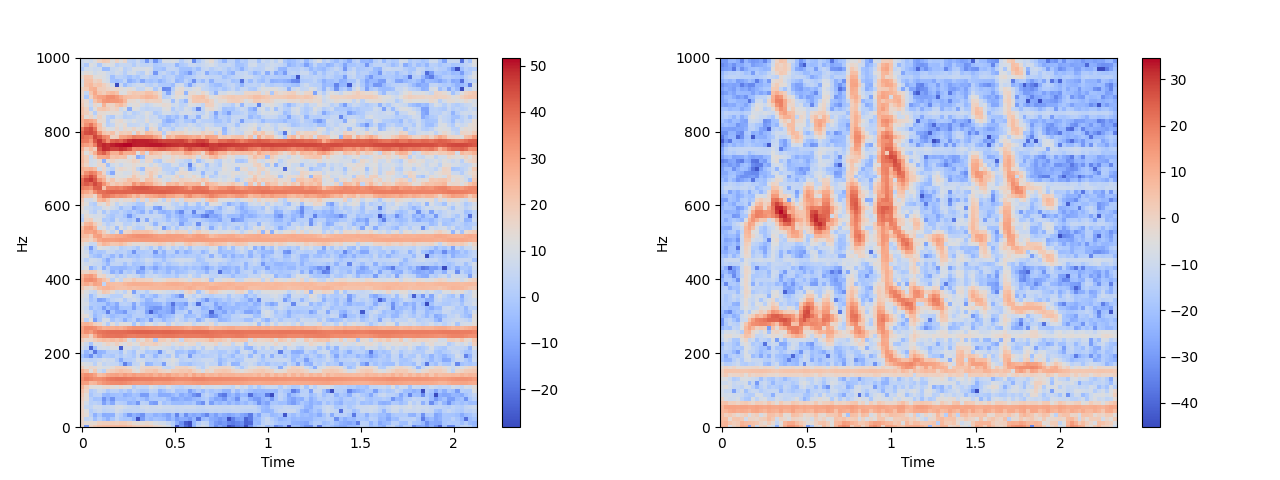
\includegraphics[width=0.8\textwidth]{wykresy/pochmara-patryk/left-male-right-female.png}
\caption{Porównanie nagrania męskiego 'A' i damskiego gadania}
\end{figure}

\newpage

\section{Kompresja dźwięku}
\label{sec:kompresja}

Kompresja danych to metoda reprezentacji informacji używając mniejszej ilości pamięci komputerowej niż oryginalna reprezentacja. Kompresję możemy podzielić na stratną i bezstratną. Stratna kompresja polega na niedokładnym przybliżeniach i częściowym odrzuceniu danych w celu reprezentacji przybliżenia informacji, podczas bezstratna kompresja pozwala na dokładną rekonstrukcje informacji. W raporcie opisana zostanie kompresja pod kątem reprezentacji dźwięku.

\addcontentsline{toc}{section}{Kompresja bezstratna}
\section*{Kompresja bezstratna}

Kompresja bezstratna pozwala na dokładną rekonstrukcje kodowanej informacji. Zazwyczaj polega na podzieleniu informacji na powtarzające się symbole i reprezentacji symboli przez słowa kodowe, których reprezentacja binarna jest krótsza dla symboli częściej występujących w kompresowanej informacji i dłuższa dla symboli występujących rzadziej.

Do najbardziej popularnych metod bezstratnej kompresji dźwięku należy Free Lossless Audio Codec (FLAC), Apple Lossless Audio Codec (ALAC) i Windows Media Audio Lossless (WMAL).

\subsection*{Przykładowy algorytm kompresji bezstratne dźwięku na przykładzie metody FLAC:}
FLAC jest metodą kompresji specjalnie zaprojektowaną do kompresji dźwięku, więc jest w stanie zmniejszyć rozmiar pliku reprezentującego dźwięk bardziej efektywnie niż uniwersalne algorytmy, których celem jest zmniejszenie rozmiaru pliku nieskompresowanego dźwięku używając np. algorytmu Huffmana.
Kodowanie FLAC polega na podzieleniu dźwięku na odcinki czasu, zwane blokami. Algorytm następnie używając interpolacji tworzy wielomian będący przybliżeniem sygnału fali dźwiękowej zawartej w bloku. W końcu różnica pomiędzy sygnałem kodowanym i sygnałem z wielomianu jest otrzymana i zakodowana przy pomocy algorytmu Golomba.

\addcontentsline{toc}{section}{Kompresja stratna}
\section*{Kompresja stratna}

Kompresja stratna w ramach kompresji dźwięku pozwala na znaczne zmniejszenie rozmiaru pliku dźwięku poprzez odrzucenie części danych, otrzymując przybliżenie zakodowanej informacji. Proces odrzucania danych zazwyczaj ma na celu odrzucenie danych mniej krytycznych, czyli sygnał wyjściowy stara się być dla człowieka percepcyjnie identyczny do sygnału kodowanego. Dziedziną zajmującą się badaniem i opisywaniem związków zachodzących pomiędzy bodźcem w postaci fali dźwiękowej, a odczuwalnym wrażeniem dźwięku, jest psychoakustyka.

Żeby osiągnąć w ramach kompresji sygnał percepcyjnie identyczny, wykorzystuje się ograniczenia człowieka w percepcji dźwięku. Podstawowym ograniczeniem percepcji człowieka w odbieraniu dźwięku jest zasięg słuchu człowieka zawierający się pomiędzy 20 Hz do 20 kHz, więc dźwięk o częstotliwościach wyższych niż 20 kHz możemy uznać za niekrytyczny. Innym efektem w psychoakustyce jest efekt przysłaniania dźwięków przez inne dźwięki. Dźwięk głośny będzie miał efekt przysłaniania dźwięków cichych w tym samym momencie czasu, ale także zauważono efekt czasowego przysłaniania dźwięków cichych przez dźwięki głośnie, to znaczy, że bezpośrednio przed doświadczeniem głośnego dźwięku, jak i po, człowiek nie postrzega dźwięków cichych. Przysłanianie czasowe jest efektem często wykorzystywanym w kompresji dźwięku.

\addcontentsline{toc}{section}{Porównanie wybranych metod kompresji}
\section*{Porównanie wybranych metod kompresji}

W tej sekcji porównane zostaną wybrane metody kompresji plików audio. Do porównania wybrane zostały metoda kompresji bezstratnej FLAC, i dwie metody kompresji stratnej MP3 i WMA (Windows Media Audio). Pliki poddane kompresji były w oryginalnym nieskompresowanym formacie WAV. Do kompresji kodekiem FLAC użyte zostały ustawienia poziomu 6 (poziom 1 - najszybsza kompresja, ale większy rozmiar pliku, poziom 8 - najwolniejsza kompresja, ale mniejszy rozmiar pliku). Przy kompresji przy użyciu kodeka MP3 (MPEG-2 Audio Layer III) wybrany został bit rate na poziomie 145-185 kbps, a przy kompresji używając kodeka FFmpeg do formatu WMA wybrany został bit rate o wymiarze 128 kbps.
Poniżej w tabeli przedstawione zostały wyniki porównania rozmiarów plików w kb przed kompresją, przedstawione w kolumnie opisanej WAV, rozmiary plików w kb po kompresji i ilorazy rozmiaru plików po kompresji i przed kompresją.

\begin{center}
\resizebox{\textwidth}{!}{
\begin{tabular}{ |c|c|c|c|c|c|c|c| } 
 \hline
Nazwa pliku & WAV & FLAC & FLAC/WAV & MP3 & MP3/WAV & WMA & WMA/WAV \\
 \hline
female-audacity-high-100 & 224 & 120 & 54\% & 22 & 10\% & 23 & 10\% \\
female-audacity-high-101 & 332 & 184 & 55\% & 32 & 10\% & 35 & 11\% \\
female-audacity-high-102 & 246 & 130 & 53\% & 25 & 10\% & 26 & 11\% \\
female-audacity-high-103 & 212 & 113 & 53\% & 22 & 10\% & 23 & 11\% \\
female-audacity-low-100 & 273 & 144 & 53\% & 26 & 10\% & 29 & 11\% \\
female-audacity-low-101 & 304 & 161 & 53\% & 29 & 10\% & 32 & 11\% \\
female-audacity-low-102 & 205 & 107 & 52\% & 21 & 10\% & 23 & 11\% \\
female-audacity-normal-100 & 197 & 104 & 53\% & 20 & 10\% & 23 & 12\% \\
female-audacity-normal-101 & 269 & 142 & 53\% & 26 & 10\% & 29 & 11\% \\
female-audacity-normal-102 & 404 & 212 & 52\% & 39 & 10\% & 42 & 10\% \\
female-audacity-normal-103 & 242 & 126 & 52\% & 24 & 10\% & 26 & 11\% \\
female-audacity-normal-104 & 858 & 444 & 52\% & 82 & 10\% & 85 & 10\% \\
male-audacity-normal-100 & 172 & 158 & 92\% & 31 & 18\% & 32 & 19\% \\
male-discord-high-0 & 301 & 147 & 49\% & 27 & 9\% & 32 & 11\% \\
male-discord-high-1 & 133 & 56 & 42\% & 10 & 8\% & 17 & 13\% \\
male-discord-high-2 & 263 & 114 & 43\% & 17 & 6\% & 29 & 11\% \\
male-discord-high-3 & 493 & 234 & 47\% & 47 & 10\% & 51 & 10\% \\
male-discord-low-0 & 235 & 111 & 47\% & 46 & 20\% & 26 & 11\% \\
male-discord-low-1 & 398 & 153 & 38\% & 26 & 7\% & 42 & 11\% \\
male-discord-low-2 & 481 & 223 & 46\% & 47 & 10\% & 51 & 11\% \\
male-discord-low-3 & 831 & 386 & 46\% & 86 & 10\% & 82 & 10\% \\
male-discord-normal-0 & 307 & 107 & 35\% & 25 & 8\% & 32 & 10\% \\
male-discord-normal-1 & 309 & 123 & 40\% & 41 & 13\% & 32 & 10\% \\
male-discord-normal-2 & 368 & 142 & 39\% & 24 & 7\% & 39 & 11\% \\
male-discord-normal-101 & 2264 & 826 & 36\% & 201 & 9\% & 223 & 10\% \\
 & & Średnia: & 49\% & Średnia: & 10\% & Średnia: & 11\%\\
 \hline
\end{tabular}}
\end{center}

\begin{figure}[h!]
\centering
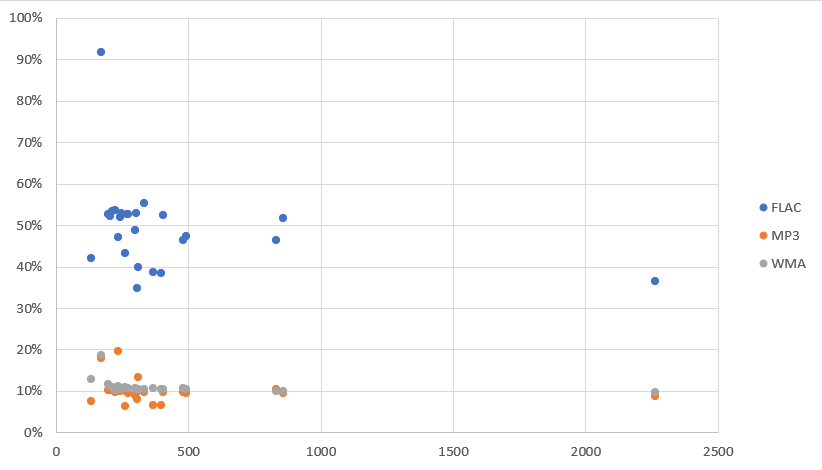
\includegraphics[width=0.75\textwidth]{wykresy/sarwinski-wojciech/Wykres kompresja.png}
\caption{Wykres iloczynów rozmiaru skompresowanego pliku do pliku nieskompresowanego używając różnych algorytmów kompresji do rozmiaru pliku nieskompresowanego}
\end{figure}

Sygnały dźwiękowe wybrane do kompresji stanowiły nagrania ludzkiego głosu. Można było zauważyć, że sygnał otrzymany każdą metodą kompresji był percepcyjne identyczny do sygnału kompresowanego. Metoda kompresji bezstratnej była w stanie zmniejszyć rozmiary plików średnio o połowę, a obie metody kompresji stratnej były w stanie zmniejszyć rozmiar pliku do ok. 10\% ich oryginalnego rozmiaru.

\newpage

\section{Własny algorytm kompresujący}
\label{sec:wlasny}

\addcontentsline{toc}{section}{Opis sekcji}
\section*{Opis sekcji}

W tej części raportu opiszę proces tworzenia własnego algorytmu kompresującego. Następnie porównam jego wyniki w różnych stadiach rozwoju oraz z innymi algorytmami. Należy zauważyć, że jest to algorytm stratny i użyteczny wyłącznie, gdy określamy częstotliwość pierwszej harmonicznej. Traci on na tyle dużo danych, że chociażby odsłuchanie pliku dźwiękowego staje się niemożliwe.

\addcontentsline{toc}{section}{Powód powstania}
\section*{Powód powstania}

Podczas gromadzenia danych zauważyłem, że potrzebna jest tylko niewielka cześć danych z zebranych próbek. Pozostała część nie wnosi żadnej informacji. Wtedy powstał pomysł stworzenia własnego algorytmu kompresującego wyłącznie na nasz użytek, który w znacznym zmniejsza redundancję.

\addcontentsline{toc}{section}{Pierwszy etap algorytmu kompresującego}
\section*{Pierwszy etap algorytmu kompresującego}

Podczas części, gdzie zbieramy dane zdecydowaliśmy się na magazynowanie plików dźwiękowych o rozszerzeniu wave. Jego zaletą jest bezstratna jakość, wiąże się to z większą objętością zbioru danych. Plik wave jest w zasadzie wektorem danych, które układają się na kształt sinusoidalny. Nasz algorytm tworzący spektrogram używa szybkiej transformaty Furiera w celu rozbicia sinusoidy na kolejne częstotliwości harmoniczne. Częstotliwość głosu człowieka, praktycznie nigdy nie przekracza 500 Hz, dlatego wystarczy użyć próbkowania o częstotliwości 1000 Hz \cite{aliasing}. W tej części algorytmu zmieniam próbkowanie na 1000 Hz. Jako sposobu gromadzenia informacji, nie używam formatu wave. Został on zastąpiony rozszerzeniem .npy, gdzie trzymam już dwuwymiarową tablice wartości dźwięku (spektrogram).

\clearpage

\begin{figure}[h!]
\centering
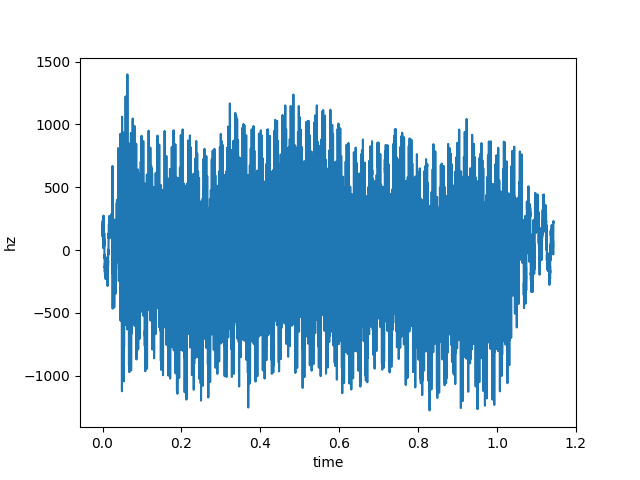
\includegraphics[width=0.75\textwidth]{wave-wide}
\caption{Sinusoidalny wykres odczytanego pliku wave (cały)}
\end{figure}

\begin{figure}[h!]
\centering
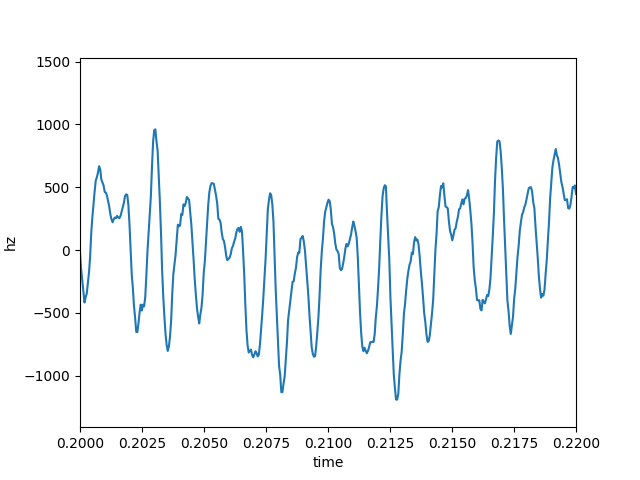
\includegraphics[width=0.75\textwidth]{wave-narrow}
\caption{Sinusoidalny wykres odczytanego pliku wave (od 0.2 do 0.22 sekundy)}
\end{figure}

\clearpage

\begin{figure}[h!]
\centering
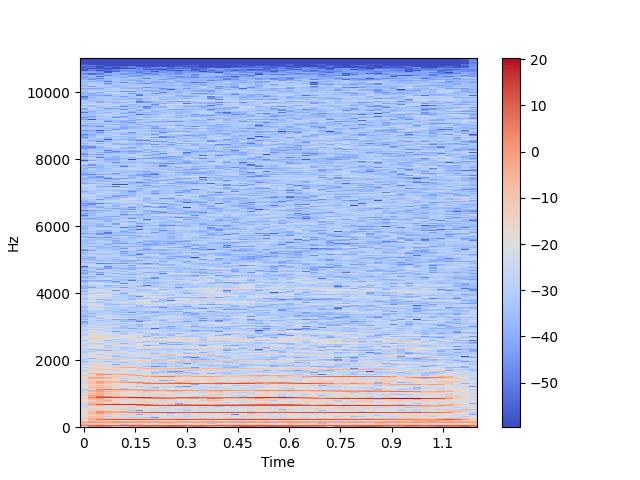
\includegraphics[width=0.75\textwidth]{spec-ylim-11025}
\caption{Spektrogram o próbkowaniu 22050 Hz, całe pasmo}
\end{figure}

\begin{figure}[h!]
\centering
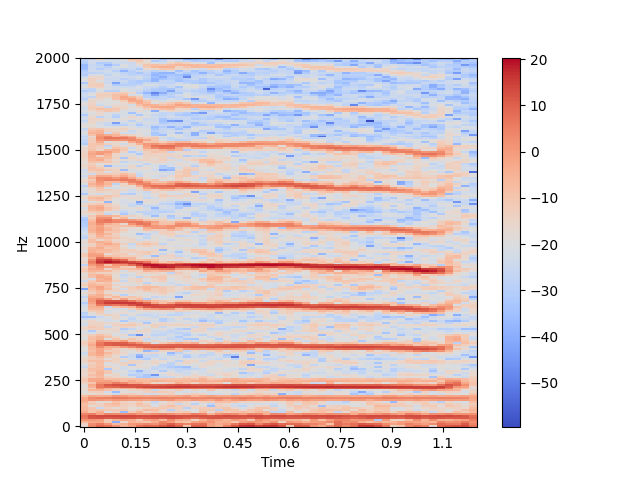
\includegraphics[width=0.75\textwidth]{spec-ylim-2000}
\caption{Spektrogram o próbkowaniu 22050 Hz, przycięty do 2000 Hz}
\end{figure}

\clearpage

\begin{figure}[h!]
\centering
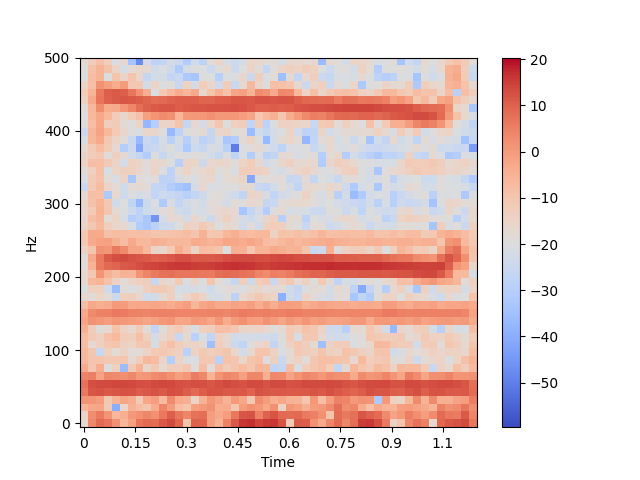
\includegraphics[width=0.75\textwidth]{spec-ylim-500}
\caption{Spektrogram o próbkowaniu 22050 Hz, przycięty do 500 Hz}
\end{figure}

\begin{figure}[h!]
\centering
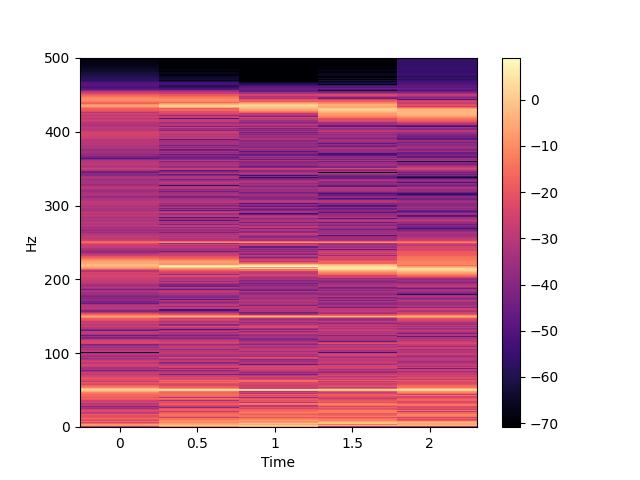
\includegraphics[width=0.75\textwidth]{spec-sr-1000}
\caption{Spektrogram o próbkowaniu 1000 Hz}
\end{figure}

\clearpage

\addcontentsline{toc}{section}{Drugi etap algorytmu kompresującego}
\section*{Drugi etap algorytmu kompresującego}

Na spektrogramie cisza nie ma wartości 0 DB. Są to wartości ujemne, które nie reprezentują żadnej informacji (w rozumieniu naszego projektu). Obcinam zatem zakres wartości dolną granicą równą 0. Następnie zauważyłem, że wszelkie szmery również stanowią nadmiarową redundancję. Między kolejnymi harmonicznymi znajduje się dużo bladych punktów. Sprawdzam jaka jest maksymalna wartość dźwięku i usuwam wszystkie wartości, które są poniżej 1/3 tej wartości. Taki parametr uznałem za najlepszy po dużej liczbie testów. Szukałem jak największej wartości, która nie zakłamuje danych. Mam teraz zakres wartości od 1/3 MAX\_DB do MAX\_DB. Aby wyzerować sporą część wykresu odejmuję od jego każdego punktu 1/3 MAX\_DB. Końcowy zakres wartości jaki używałem mieści się między 0, a 2/3 MAX\_DB. Należy zauważyć, że w dwuwymiarowej macierzy znajduje się bardzo dużo zer. Znacząco obniży to zajmowane miejsce w czasie kompresji ZIP. O tym napiszę w innej części raportu. Wartości dźwięku mieszą się między 0, a kilkudziesięcioma decybelami. Są one zapisane jako typ double. Zajmuje on 8 bajtów pamięci. Jest to duże marnotrawstwo pamięci. Zamieniłem tym danych w macierzy na bajtowe liczby całkowite typu unsigned (tylko wartości nieujemne). Dzięki zmianie typu zmiennych zaoszczędziłem 8-krotnie więcej pamięci.

\clearpage

\begin{figure}[h!]
\centering
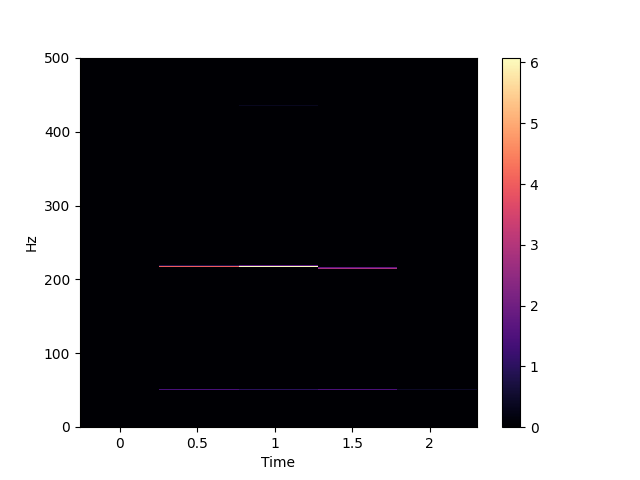
\includegraphics[width=0.75\textwidth]{spec-trimmed}
\caption{Spektrogram o uciętych wartościach}
\end{figure}

\begin{figure}[h!]
\centering
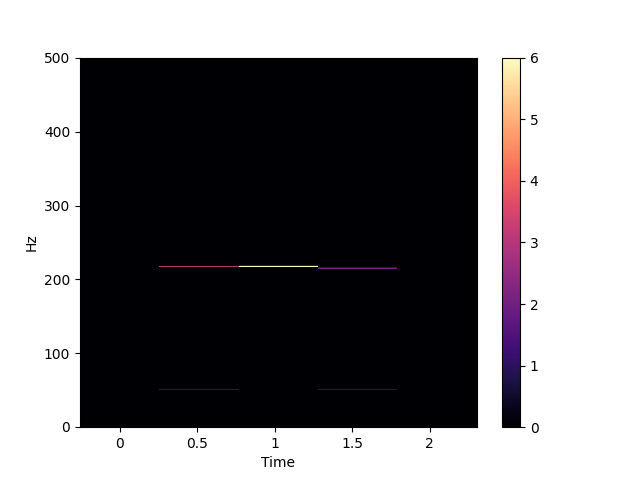
\includegraphics[width=0.75\textwidth]{spec-uint8}
\caption{Spektrogram o całkowitych wartościach}
\end{figure}

\clearpage

\addcontentsline{toc}{section}{Trzeci etap algorytmu kompresującego}
\section*{Trzeci etap algorytmu kompresującego}

Kolejne harmoniczne spektrogramu nie są pojedynczymi liniami. Są one rozciągnięte wzdłuż osi OY. Wynika to specyfiki sprzętu nagrywającego. Człowiek tworzy dźwięki o konkretnej częstotliwości, lecz podczas próbkowania zniekształca się rozciągając na szersze spektrum. Stworzyłem algorytm ściskający potencjalną częstotliwość harmoniczną. Sprawdza on czy nie natrafił na ciąg liczb niezerowych. Sprawdza ich średnią arytmetyczną i nadpisuje środkowy wyraz wynikiem, zerując pozostałe. Dzięki takiemu uszczupleniu zbędne rozciągnięcie jest usuwane.

\begin{figure}[h!]
\centering
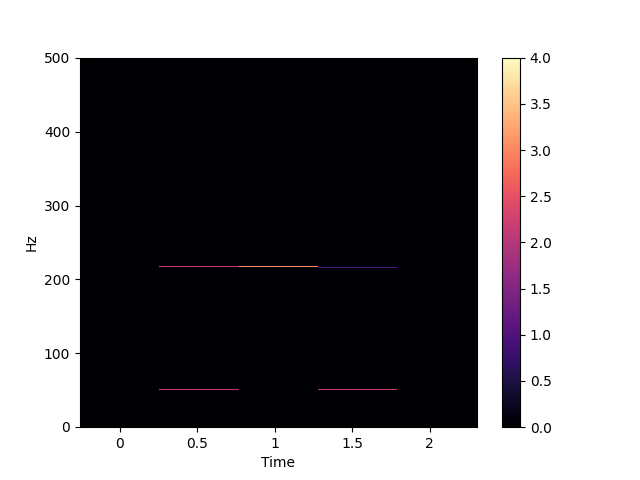
\includegraphics[width=0.75\textwidth]{spec-squeezed}
\caption{Spektrogram o ściśniętych harmonicznych}
\end{figure}

\clearpage

\addcontentsline{toc}{section}{Czwarty etap algorytmu kompresującego}
\section*{Czwarty etap algorytmu kompresującego}

Macierz danych ma niezwykle dużo zer (dzięki poprzednim etapom). Możemy wykorzystać tą informację i zastosować algorytm kompresujący. Zbędne jest trzymanie zera na całym bajcie. Użyję tutaj algorytmu kompresującego ZIP, który pobiera moją dwuwymiarową macierz i zapisuje ją w sposób zoptymalizowany. Aby zobrazować część jego działania posłużę się przykładem. Załóżmy, że mamy macierz

$$
\begin{bmatrix}
4 & 9 & 7\\
0 & 0 & 0\\
0 & 0 & 0\\
0 & 3 & 5
\end{bmatrix}
$$

\noindent Zamiast trzymania wszystkich danych, możemy zapamiętać tylko pierwszy i ostatni rząd. Wiemy, że pozostałe są zerowe. Taka kompresja przy naszej dwuwymiarowej tablicy, gdzie większość danych się wyzerowała jest idealnym wyborem. Na tym etapie kończy się działanie algorytmu kompresującego.

\begin{figure}[h!]
\centering
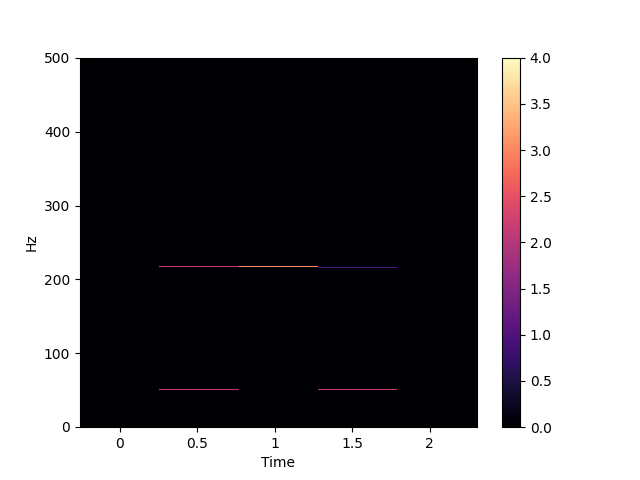
\includegraphics[width=0.8\textwidth]{spec-zip}
\caption{Spektrogram o po archiwizacji ZIP (niezmieniony)}
\end{figure}

\clearpage

\addcontentsline{toc}{section}{Porównanie kompresji kolejnych etapów}
\section*{Porównanie kompresji kolejnych etapów}

W tej sekcji porównam ilość zaoszczędzonego miejsca, między kolejnymi etapami kompresji. Własnego algorytmu kompresującego nie porównam z innymi algorytmami kompresującymi pliki dźwiękowe, gdyż takowe nie ma sensu. Jest to nieuczciwe spojrzenie na informację, dającą mi zasadniczą przewagę. Patrząc na plik dźwiękowy uniwersalnie, moja kompresja praktycznie całkowicie usuwa informację. Nie można chociażby otworzyć z niej pliku dźwiękowego. Służy on wyłącznie w celu uzyskaniu kolejnych harmonicznych. Należy jednak podkreślić, że nie trzymam surowej pierwszej harmonicznej. Powstały wykres jest nadal tym samym spektrogramem, lecz z mniejszą ilością danych, które były zbędne. Wszystkie dane liczbowe podane są w bajtach.

\clearpage

\newgeometry{left=2cm,top=2cm}

\section*{Tabela wyników}

\begin{table}[!ht]
\centering
    \resizebox{\textwidth}{!}{%
    \begin{tabular}{|l|l|l|l|l|l|l|}
    \hline
        Nazwa pliku & Oryginał [B] & Etap 1 [B] & Etap 2 [B] & Etap 3 [B] & Etap 4 [B] & Wskaźnik \\ \hline
        male-discord-normal-103.wav & 215108 & 10388 & 2693 & 2693 & 283 & 99.87 \\ \hline
        male-discord-high-2.wav & 268840 & 12440 & 3206 & 3206 & 340 & 99.87 \\ \hline
        male-twitch-normal-0.wav & 1121212 & 51428 & 12953 & 12953 & 350 & 99.97 \\ \hline
        female-iphone-normal-102.wav & 186518 & 18596 & 4745 & 4745 & 326 & 99.83 \\ \hline
        male-youtube-normal-0.wav & 354016 & 16544 & 4232 & 4232 & 584 & 99.84 \\ \hline
        male-discord-normal-1.wav & 315436 & 14492 & 3719 & 3719 & 365 & 99.88 \\ \hline
        male-discord-low-2.wav & 491672 & 22700 & 5771 & 5771 & 367 & 99.93 \\ \hline
        male-discord-normal-0.wav & 313388 & 14492 & 3719 & 3719 & 414 & 99.87 \\ \hline
        female-audacity-high-101.wav & 339904 & 16544 & 4232 & 4232 & 293 & 99.91 \\ \hline
        female-audacity-low-102.wav & 209848 & 10388 & 2693 & 2693 & 279 & 99.87 \\ \hline
        female-iphone-normal-103.wav & 388028 & 37064 & 9362 & 9362 & 427 & 99.89 \\ \hline
        male-discord-low-3.wav & 850072 & 39116 & 9875 & 9875 & 419 & 99.95 \\ \hline
        female-audacity-normal-104.wav & 878124 & 41168 & 10388 & 10388 & 435 & 99.95 \\ \hline
        female-discord-low-100.wav & 150560 & 8336 & 2180 & 2180 & 278 & 99.82 \\ \hline
        male-discord-normal-101.wav & 2317940 & 106832 & 26804 & 26804 & 329 & 99.99 \\ \hline
        female-iphone-normal-101.wav & 160838 & 16544 & 4232 & 4232 & 315 & 99.8 \\ \hline
        female-iphone-high-100.wav & 246190 & 22700 & 5771 & 5771 & 375 & 99.85 \\ \hline
        female-twitch-normal-0.wav & 915500 & 43220 & 10901 & 10901 & 280 & 99.97 \\ \hline
        female-audacity-normal-100.wav & 201716 & 10388 & 2693 & 2693 & 297 & 99.85 \\ \hline
        male-discord-high-0.wav & 307244 & 14492 & 3719 & 3719 & 308 & 99.9 \\ \hline
        male-discord-high-3.wav & 504472 & 24752 & 6284 & 6284 & 370 & 99.93 \\ \hline
        male-audacity-normal-100.wav & 310352 & 14492 & 3719 & 3719 & 324 & 99.9 \\ \hline
        male-discord-normal-2.wav & 376728 & 18596 & 4745 & 4745 & 361 & 99.9 \\ \hline
        female-audacity-normal-101.wav & 275168 & 14492 & 3719 & 3719 & 322 & 99.88 \\ \hline
        female-twitch-normal-1.wav & 1140468 & 53480 & 13466 & 13466 & 397 & 99.97 \\ \hline
        female-iphone-low-101.wav & 89824 & 8336 & 2180 & 2180 & 300 & 99.67 \\ \hline
        female-audacity-high-100.wav & 228944 & 12440 & 3206 & 3206 & 290 & 99.87 \\ \hline
        female-discord-normal-100.wav & 107960 & 6284 & 1667 & 1667 & 272 & 99.75 \\ \hline
        female-audacity-low-101.wav & 311272 & 14492 & 3719 & 3719 & 345 & 99.89 \\ \hline
        female-discord-high-100.wav & 175168 & 8336 & 2180 & 2180 & 260 & 99.85 \\ \hline
        female-iphone-normal-100.wav & 122192 & 12440 & 3206 & 3206 & 299 & 99.76 \\ \hline
        male-discord-low-1.wav & 406672 & 20648 & 5258 & 5258 & 425 & 99.9 \\ \hline
        male-discord-normal-102.wav & 1245328 & 57584 & 14492 & 14492 & 340 & 99.97 \\ \hline
        male-discord-normal-4.wav & 425936 & 20648 & 5258 & 5258 & 503 & 99.88 \\ \hline
        male-iphone-normal-100.wav & 247786 & 22700 & 5771 & 5771 & 595 & 99.76 \\ \hline
        female-iphone-high-102.wav & 221334 & 20648 & 5258 & 5258 & 302 & 99.86 \\ \hline
        female-iphone-high-101.wav & 336022 & 30908 & 7823 & 7823 & 329 & 99.9 \\ \hline
        female-audacity-high-103.wav & 216796 & 10388 & 2693 & 2693 & 281 & 99.87 \\ \hline
        female-audacity-normal-103.wav & 247364 & 12440 & 3206 & 3206 & 292 & 99.88 \\ \hline
        male-discord-normal-3.wav & 441388 & 20648 & 5258 & 5258 & 309 & 99.93 \\ \hline
        male-discord-low-100.wav & 235920 & 12440 & 3206 & 3206 & 277 & 99.88 \\ \hline
        male-discord-high-1.wav & 135212 & 6284 & 1667 & 1667 & 258 & 99.81 \\ \hline
        female-iphone-normal-104.wav & 209046 & 20648 & 5258 & 5258 & 366 & 99.82 \\ \hline
        female-iphone-low-100.wav & 139728 & 14492 & 3719 & 3719 & 310 & 99.78 \\ \hline
        female-audacity-normal-102.wav & 412708 & 20648 & 5258 & 5258 & 335 & 99.92 \\ \hline
        male-youtube-normal-4.wav & 629288 & 28856 & 7310 & 7310 & 324 & 99.95 \\ \hline
        female-audacity-high-102.wav & 251528 & 12440 & 3206 & 3206 & 286 & 99.89 \\ \hline
        male-iphone-normal-101.wav & 198806 & 18596 & 4745 & 4745 & 450 & 99.77 \\ \hline
        male-discord-low-0.wav & 239660 & 12440 & 3206 & 3206 & 289 & 99.88 \\ \hline
        female-audacity-low-100.wav & 279360 & 14492 & 3719 & 3719 & 322 & 99.88 \\ \hline
        ~ & ~ & ~ & ~ & ~ & Średnia & 99.87 \\ \hline
    \end{tabular}}
\end{table}

\restoregeometry

\clearpage

\addcontentsline{toc}{section}{Podsumowanie algorytmu}
\section*{Podsumowanie algorytmu}

Należy podkreślić mimo tego, że etap drugi i trzeci mają taki sam rozmiar, etap trzeci wpływa na wynik etapu czwartego. Zmniejszenie ilości danych nie zmienia sposobu w jaki biblioteka numpy zapisuje dane. Zerowy punkt w macierzy cały czas zajmuje bajt miejsca. Natomiast kompresja ZIP wykorzystuje już te zero, zmniejszając jego redundancję. Gdyby usunąć trzeci etap, miejsce zajmowane po całej kompresji zwiększyłoby się.

Końcowy wynik jest ponad zadowalający. Kompresja na poziomie wskaźnika 99.87 jest niemożliwa do osiągnięcia dla innych algorytmów kompresujących dźwięk. Zostały one opisane w sekcji dotyczącej porównania różnych kompresji dźwięku.

\clearpage

\printbibliography[title=Bibliografia]

\end{document}
